\chapter{Discussion}
\section{Comparison to a Commercial Product}
In order to get an idea of what directional characteristics have been achieved by others, the beamforming array is compared to a line array unit by the company D\&B, who specifically use their directivity control for marketing. The so called GLS8 unit is depicted in \autoref{fig:gls8_pic}. For the frequency range of this project, the key data is, that in the line array unit, two 14$^{\prime \prime}$ drivers in the front of the unit are placed, and another two 10$^{\prime \prime}$ drivers are mounted in the sides \citep{SL_GSL}[p. 6]. 
\begin{figure}[H]
\centering
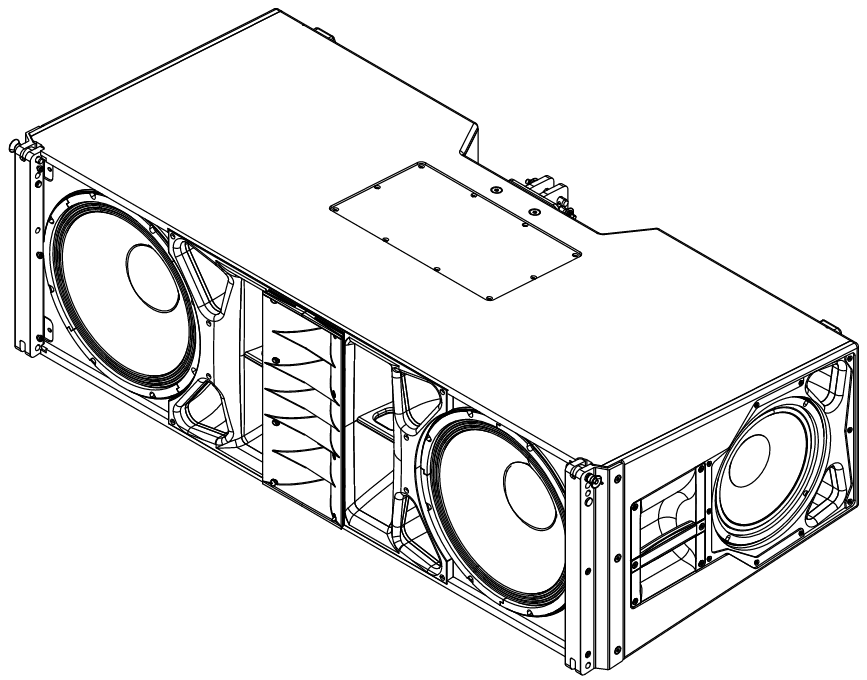
\includegraphics[width=0.4\textwidth]{sl8.png}
\caption{Drawing of D\&B GLS8 line array unit, image source: \citep{SL_GSL}[p. 6]}
\label{fig:gls8_pic}
\end{figure}
The directional characteristics of the GSL8 units are depicted in \autoref{fig:gls_iso}. 
It has to be noted that this plot covers a significantly wider frequency range, than the one featured in this project. Between \SI{200}{\hertz} and \SI{300}{\hertz}, the line array unit clearly has a smaller \SI{-6}{\decibel} lobe width (approx. \SI{80}{\degree}) than the triangular array (approx. \SI{140}{\degree}), which is featured in \autoref{fig:array_iso}.
\autoref{fig:gls_iso} shows, that the lobe width for the line array module has a tendency to grow with decreasing frequency. At \SI{63}{\hertz} the \SI{-6}{\decibel} lobe width of the GSL8 unit is approx. \SI{144}{\degree}, which is in the same order of magnitude as the approx. \SI{150}{\degree} lobe width of the triangular array. When looking at these plots it has to be taken into account, that the two constructions were designed to fulfill different requirements and have very different cabinet configurations. It might be speculated, that perhaps the relatively large single cabinet of the line array unit aids directionality at higher frequencies, where at the lower end of the frequency band more of the directionality control has to be achieved by beamforming. This would explain, why at higher frequencies the lobe width of the GSL8 is clearly superior to the triangular array, while they both have similar characteristics around \SI{60}{\hertz}.
\begin{figure}[H]
\centering
	\begin{subfigure}[H]{0.7\textwidth}
		\centering
		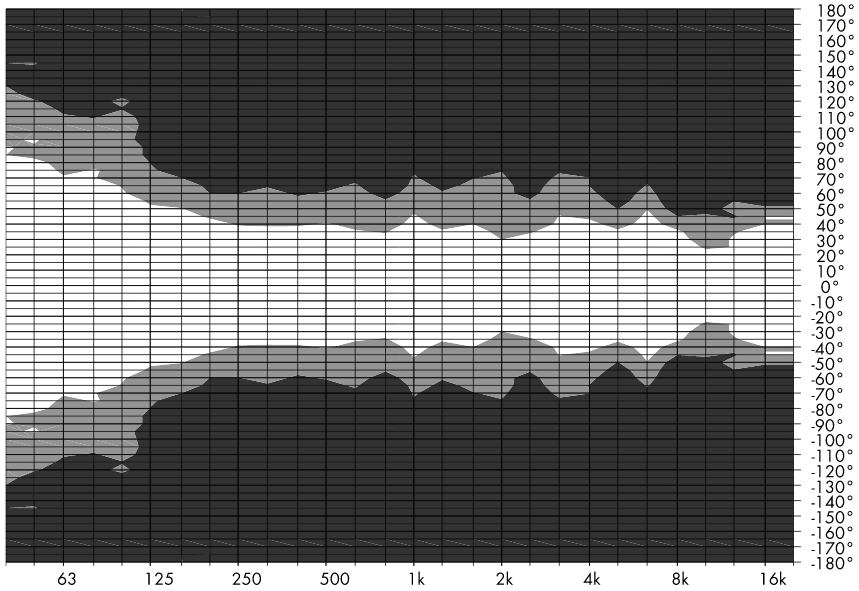
\includegraphics[width=0.95\textwidth]{gls_isobar.png}
		\subcaption{Isobar plot for the GSL8 module, showing \SI{-6}{\decibel} and \SI{-12}{\decibel} isobars, image source: \citep{SL_GSL}[p. 9]}	
		\label{fig:gls_iso}
	\end{subfigure}\\
	\begin{subfigure}[H]{0.95\textwidth}
		\centering
		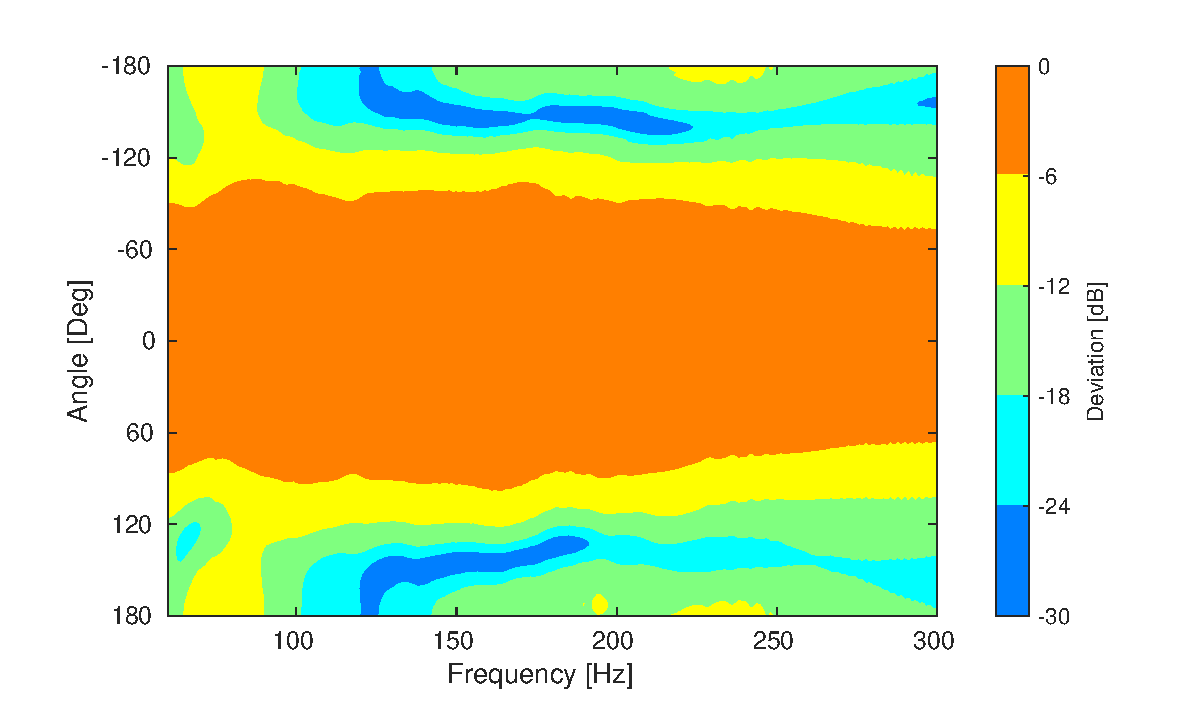
\includegraphics[width=0.95\textwidth]{dbcompare.eps}
		\subcaption{Contour plot of the relative level over frequency and angle for the triangular speaker array. Modified version of \autoref{fig:beamdwidth_array_on}, with resolution adjusted for comparison}
		\label{fig:array_iso}
	\end{subfigure}
\caption{Directional characteristics, GSL8 and triangular speaker array.}
\label{fig:isobars}
\end{figure}
\section{Applications}\label{sec:applications}
\subsection{Home application}
The beamforming array in its current form might be quite big for home applications, but it may be possible to reduce the size of the beamforming array with smaller speaker units. At this point, there are several possibile ideas for home application. Imagine a house is designed and built as an open living environment, where the kitchen and the living room are a combined into an open area. There might be a television with stereo speakers in the living room where the back for the television and therefore back of speakers points towards the kitchen. Undesired low frequency emission might be an issue, because the low frequency loudspeakers radiate omnidirectionally. At higher frequencies, there will be more sound radiated towards the persons watching television, because at higher frequencies the loudspeakers have a tendency to be cardioid in themselves, leading to mainly reflected sound making its way to kitchen. Because of this directionality, there might be higher pressure in the kitchen of the low frequency than in the high frequency. Therefore the hearing experience might be unpleasant in the kitchen, because it is dominated by low frequency sound. A simulation of an indoor situation with 2 speaker arrays in a living room is done in \autoref{fig:Indoor_simulation_60_100} and \autoref{fig:Indoor_simulation_200_300}. In the reference case, the arrays are replaced by three speakers, that are positioned in a line. It is apparent, that especially at \SI{60}{\hertz} and \SI{100}{\hertz} the sound pressure in the room in general is attenuated significantly by the speaker arrays, leading to a more even pressure distribution along the frequency band. As a drawback, modes in the room are more distinctive in the beamforming case.


\subsection{Monitoring}
Using a normal loudspeaker as a stage monitor might lead to some complications, when the monitor and the microphone create a feedback loop or the performers are annoyrd by crosstalk from the monitors of other performers. The beamforming array cannot solve the feedback loop, but using beamforming will decrease the pressure emitted towards the side of the monitor at low frequencies and might therefore reduce crosstalk. This application has potential at stages both inside and outside. The problem of using this inside can be, that reflections are so strong that the effect do not occur as intended. Another problem with monitors might be, that the stage is small and there is barely space for several monitors. By adding additional inputs and filters, the beamforming array can be used to emit different signals with different main lobes at the same time. Using this, it might be possible replace several single monitors with one beamforming array. By narrowing the width of front beam at the expense of allowing higher sound emission towards the back, it might be possible to point main lobes each of the on the performers as desired. This kind of beamforming requires further investigation and designing, which has not been covered in this project. A simulation is made of a indoor application where two monitors of the beemforming array are placed on a stage, see \autoref{sec:dis:simulation}



\subsection{Main application}
The main application of the beamforming array, that has been mentioned in the problem statement, was the use at outdoor venues, where involuntary listeners are in the vicinity. In this application, it can be assumed that the speaker array is in a soundfield with conditions reasonably close to at least a semi-free-field. It  been shown that in free-field conditions, the sound pressure can be attenuated at least \SI{-12}{\decibel} at the back of the array. Therefore the beamforming array can be used to reducing noise pollution as a side effect of outdoor concerts.


\subsection{Simulation}\label{sec:dis:simulation}
The aim of this section is to shortly investigate the behaviour of the speaker array in a sound field with wall reflections. This project so far has mainly covered the design of the beamforming array and the behaviour in free field conditions. The indoor application have been of less interest, because of the starting point of application, which has been focused on outdoor events. The last point in the problem statement is questioning the indoor behaviour of the beamforming array. For this, there are many things to be investigated, because of the innumerable amount of possible room is configurations. The room could be a big concert hall or just a small living room. It have been chosen to simulate a concert hall because of the monitoring application and the living room for home application. For the living room, it has been chosen to use a standard listening room of size (\SI{4.15}{\meter} x \SI{7.8}{\meter}) which approximately corresponds to the dimensions of the \gls{aau} standard listening room. All simulation will be done with a 2 dimensional grid, because of computation time and memory requirements. The results do not represent an exact simulation of the room, since the reflection coefficient of the walls in the room are unknown and have not been measured there are many unknown parameters in this simulation. The reflection in this simulation implemented with $Z_{-1}$ and $Z_{1}$ set to zero, resulting in a not-frequency dependend wall impedance, because in many case the characteristic wall impedance $Z_0$ is the predominant part \citep{fdtd_imp}. $Z_0$ can be approximated with using the absorbing coefficient \citep{fdtd_imp}. The following \autoref{eq:absorb} shows the approximated characteristic wall impedance $Z_0$ calculation

\begin{equation}\label{eq:absorb}
Z_0 = \rho c \frac{1+\sqrt{1-\alpha}}{1-\sqrt{1-\alpha}}
\end{equation}

        \startexplain
        \explain{$a$ is the absorbing coefficient}{\si{1}}
    \stopexplain
    
The simulation results, that are presented as follows, only give an impression of what the sound field in the room could look like. The result from a simulation the room sized like the standard listening room is shown in \autoref{fig:Indoor_simulation_60_100} and \autoref{fig:Indoor_simulation_200_300}.



\begin{figure}[H]
\begin{subfigure}[c]{0.5\textwidth}
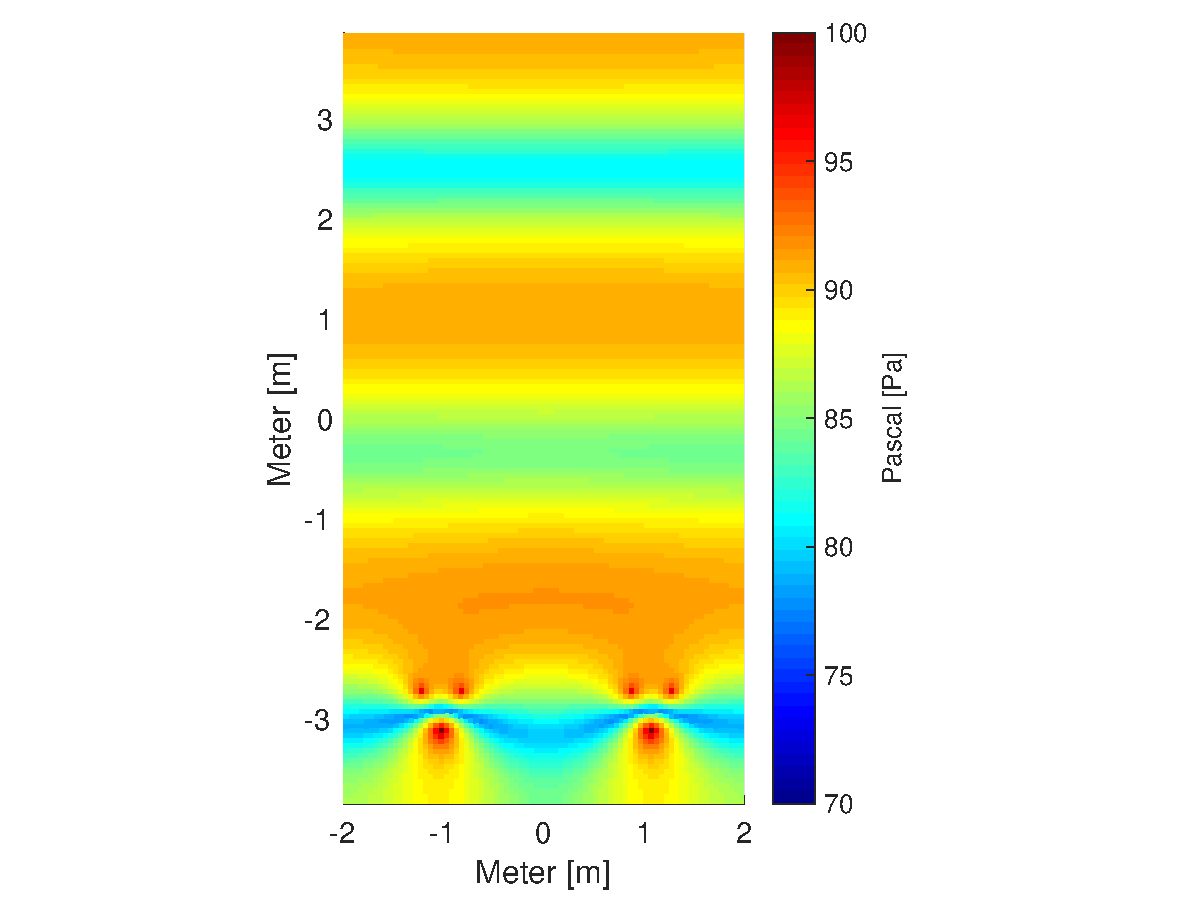
\includegraphics[width=0.95\textwidth]{60_hz_inside_beam.eps}
\subcaption{Indoor simulation of  \SI{60}{\hertz} with beamforming}
\label{fig:Indoor_simulation_60_on}
\end{subfigure}
\begin{subfigure}[c]{0.5\textwidth}
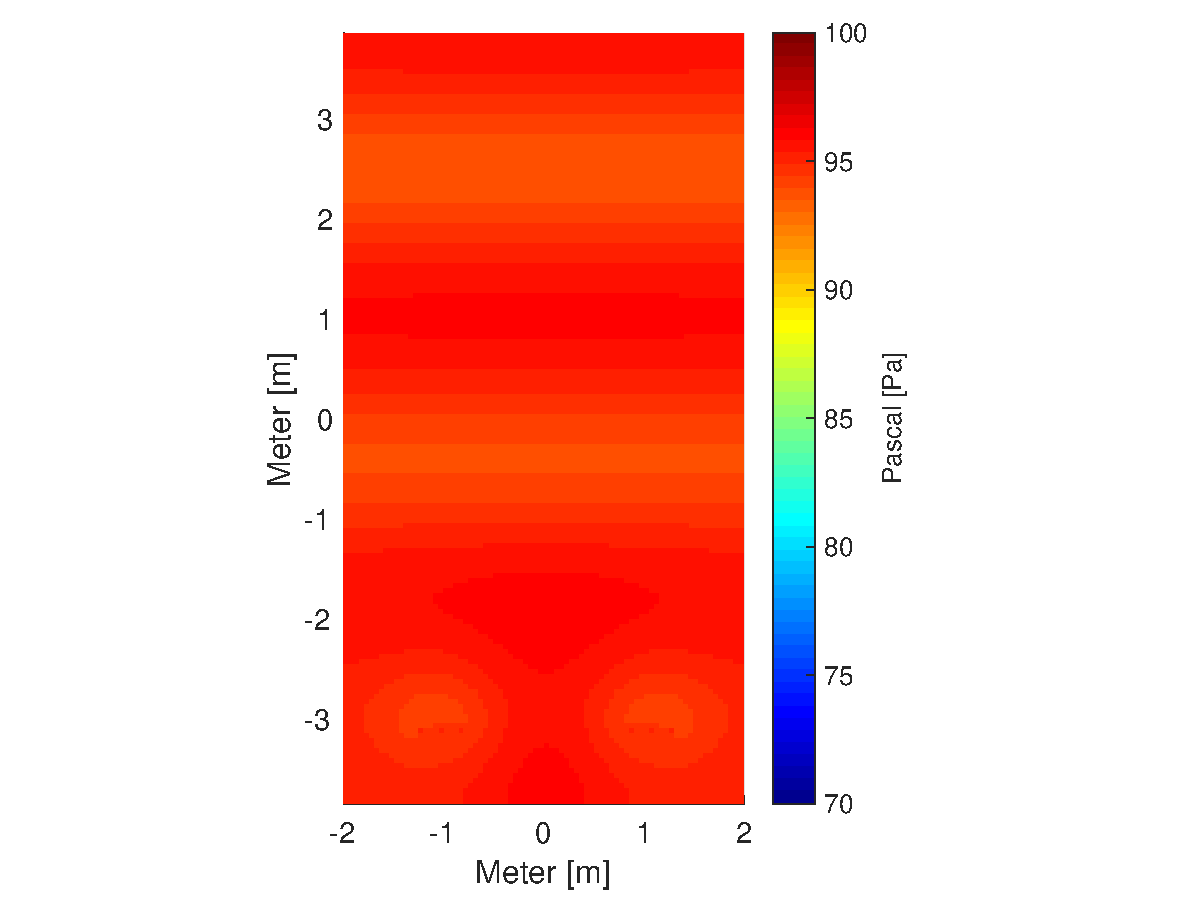
\includegraphics[width=0.95\textwidth]{60_hz_inside_without_beam.eps}
\subcaption{Indoor simulation of  \SI{60}{\hertz} without beamforming}
\label{fig:Indoor_simulation_60_off}
\end{subfigure}\\
\hspace{0.1\textheight}
\begin{subfigure}[c]{0.5\textwidth}
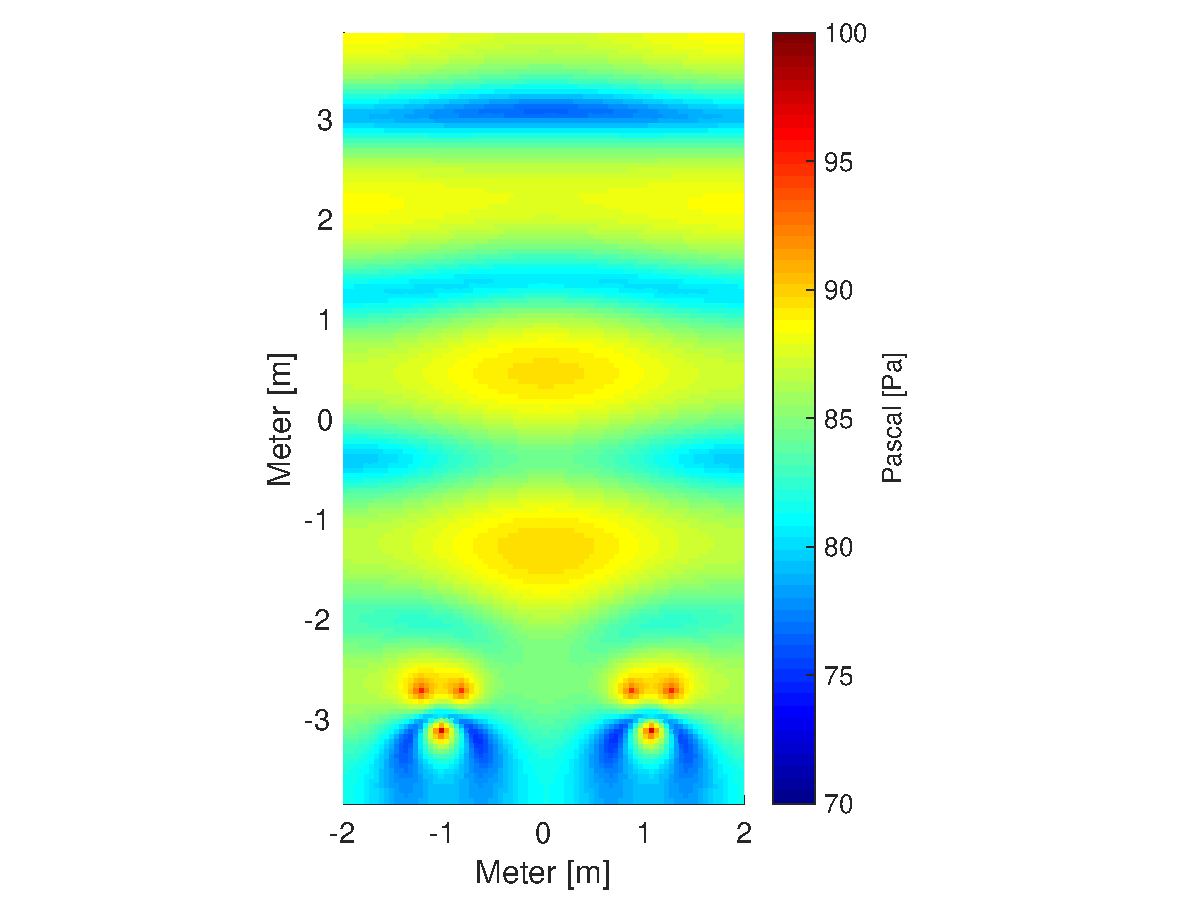
\includegraphics[width=0.95\textwidth]{100_hz_inside_beam.eps}
\subcaption{Indoor simulation of  \SI{100}{\hertz} with beamforming}
\label{fig:Indoor_simulation_100_on}
\end{subfigure}
\begin{subfigure}[c]{0.5\textwidth}
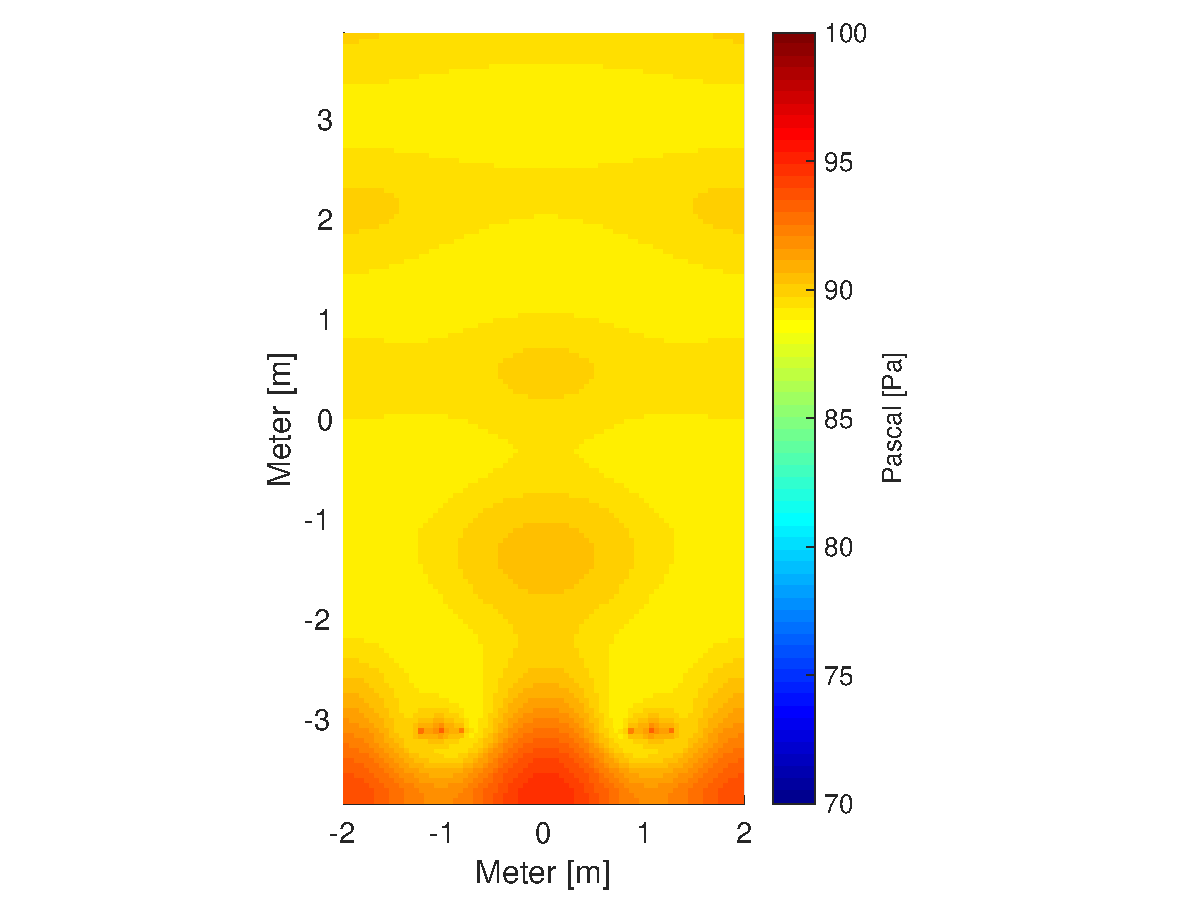
\includegraphics[width=0.95\textwidth]{100_hz_inside_without_beam.eps}
\subcaption{Indoor simulation of  \SI{100}{\hertz} with beamforming}
\label{fig:Indoor_simulation_100_off}
\end{subfigure}
\caption{The figure shows a 2 dimension \gls{fdtd} simulation in a room of size  (\SI{4.15}{\meter} x \SI{7.8}{\meter}) where the absorbing coefficient is set to 0.5}
		\label{fig:Indoor_simulation_60_100}
\end{figure}


\begin{figure}[H]
\begin{subfigure}[c]{0.5\textwidth}
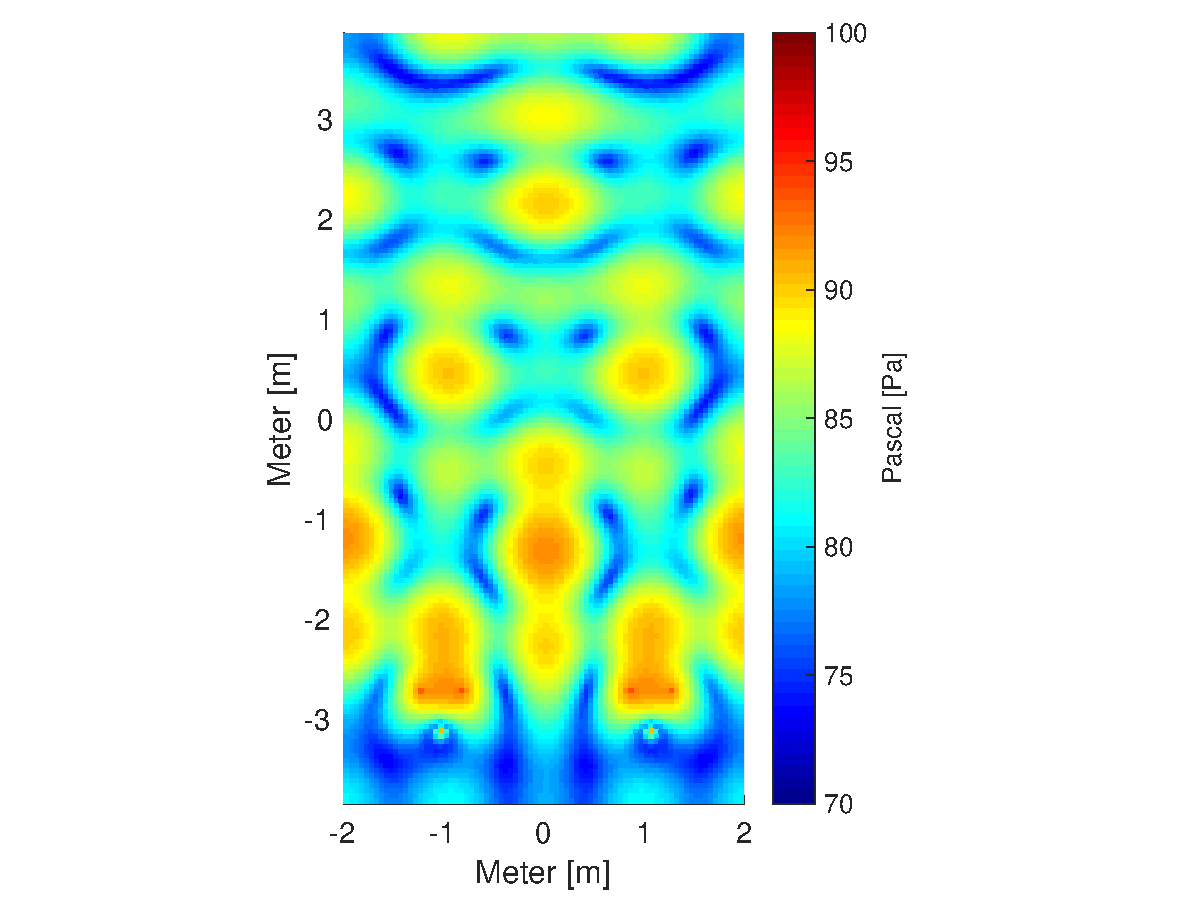
\includegraphics[width=0.95\textwidth]{200_hz_inside_beam.eps}
\subcaption{Indoor simulation of  \SI{200}{\hertz} with beamforming}
\label{fig:Indoor_simulation_200_on}
\end{subfigure}
\begin{subfigure}[c]{0.5\textwidth}
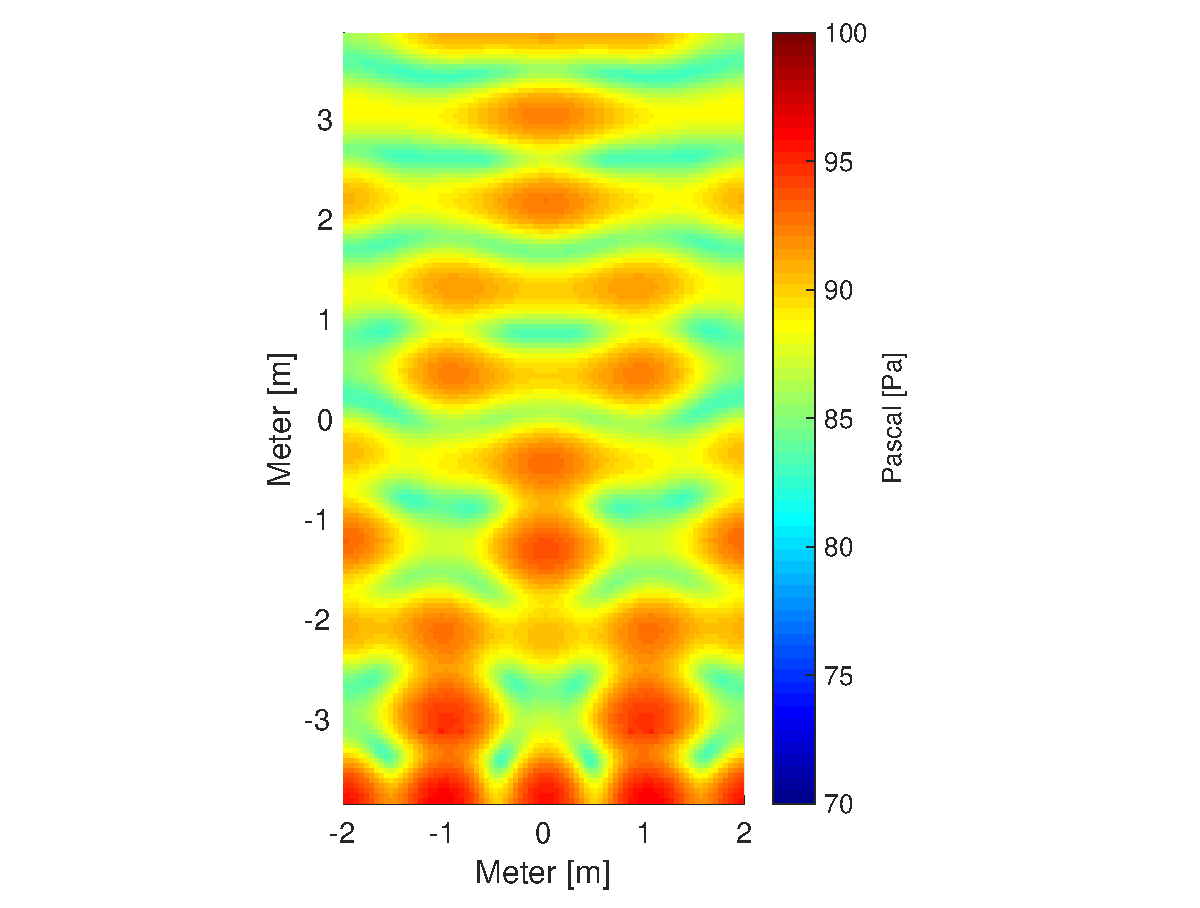
\includegraphics[width=0.95\textwidth]{200_hz_inside_without_beam.eps}
\subcaption{Indoor simulation of  \SI{200}{\hertz} without beamforming}
\label{fig:Indoor_simulation_200_off}
\end{subfigure}
\begin{subfigure}[c]{0.5\textwidth}
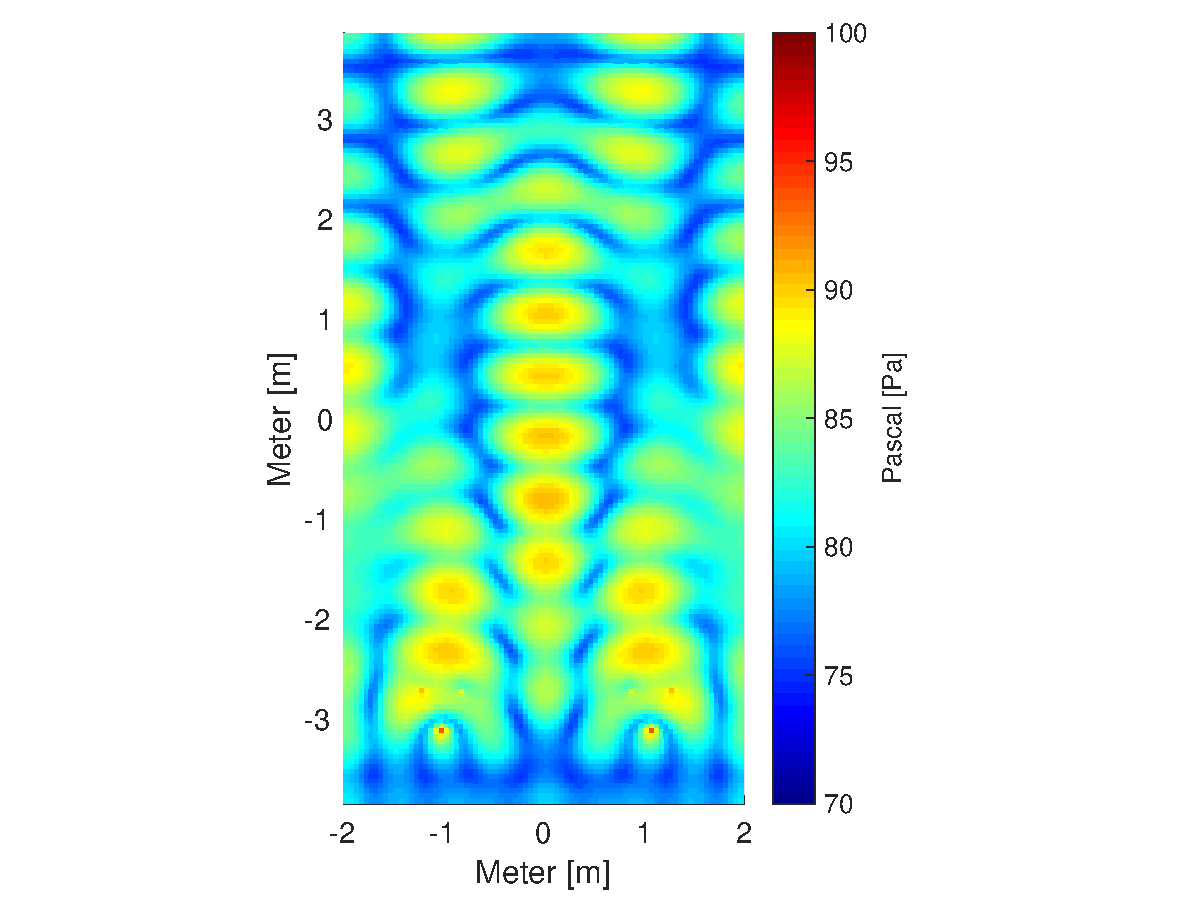
\includegraphics[width=0.95\textwidth]{300_hz_inside_beam.eps}
\subcaption{Indoor simulation of  \SI{300}{\hertz} with beamforming}
\label{fig:Indoor_simulation_300_on}
\end{subfigure}
\begin{subfigure}[c]{0.5\textwidth}
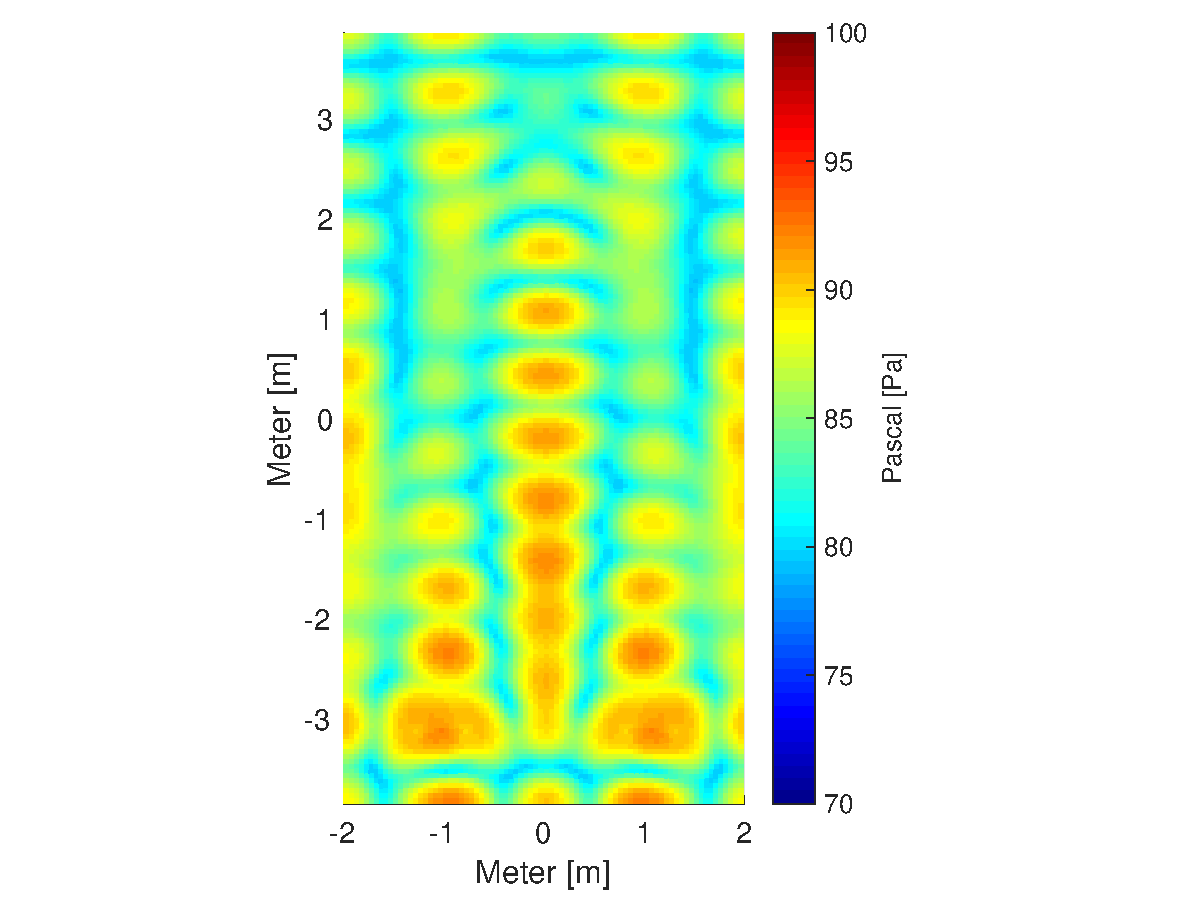
\includegraphics[width=0.95\textwidth]{300_hz_inside_without_beam.eps}
\subcaption{Indoor simulation of  \SI{300}{\hertz} without beamforming}
\label{fig:Indoor_simulation_300_off}
\end{subfigure}
\caption{The figure shows a 2 dimension \gls{fdtd} simulation in a room of size  (\SI{4.15}{\meter} x \SI{7.8}{\meter}) where the absorbing coefficient is set to 0.5}
		\label{fig:Indoor_simulation_200_300}
\end{figure}

In \autoref{fig:Indoor_simulation_60_100} and \autoref{fig:Indoor_simulation_200_300} it can be seen that the pressure in the room is not evenly distributed either with beamforming active or not. One notable thing is, that the pressure in the room at low frequency in the reference case, where the arrays have each been replaced by three speakers in a line array, gets very high compared to higher frequency.
Higher pressures build up in the room at lower frequencies without beamforming than at higher frequencies.% So the room amplify the low frequency with reflection more that in the higher frequency area. 
The average pressure in the room seems to be more consistent over the frequency range with beamforming enabled compared to the reference case.\\


The second indoor application, that shall be illustrated, is monitoring. In a monitoring application the room tends to be larger than a living room. The use of monitoring is often at both small and big concerts, where both dedicated concert hall and sports arenas are used. The following simulation examples are done in a sports arena sized room. Typically, the spectator areas at sports event are on the long sides of the playing field. A handball playing field has a size of (\SI{20}{\meter}x\SI{40}{\meter}) and in the case of the simulated room, there is space for \SI{5}{\meter} of spectator area on both long sides. The following simulation, depicted in \autoref{fig:Indoor_monitor_60_300}, shows a simulation where a stage is placed on the short side of the arena and two monitoring arrays are simulated. Both monitors are playing in the upwards direction when looking at the simulation.


\begin{figure}[H]
\begin{subfigure}[c]{0.5\textwidth}
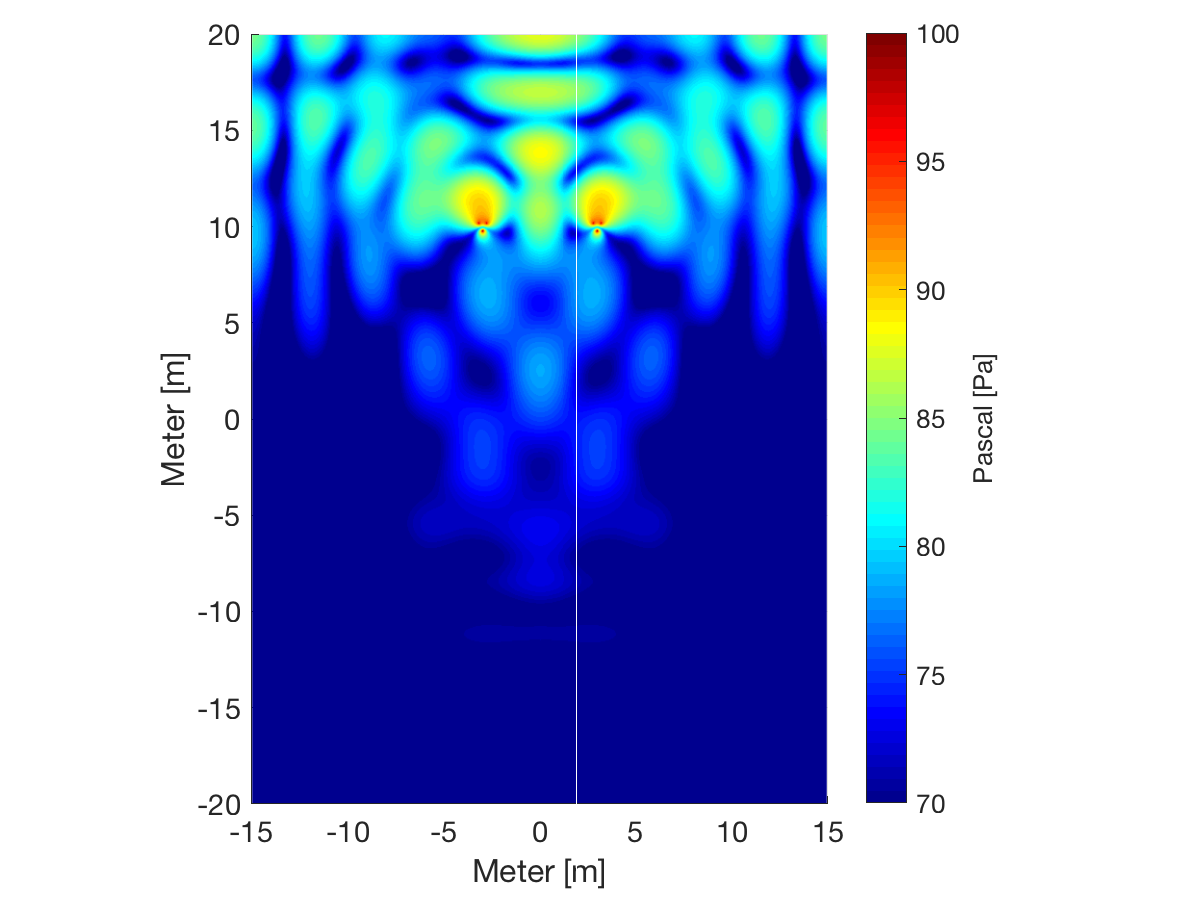
\includegraphics[width=0.95\textwidth]{60_hz_monitor_beam.eps}
\subcaption{Indoor simulation of  \SI{60}{\hertz} with beamforming}
\label{fig:Indoor_monitor_60_on}
\end{subfigure}
\begin{subfigure}[c]{0.5\textwidth}
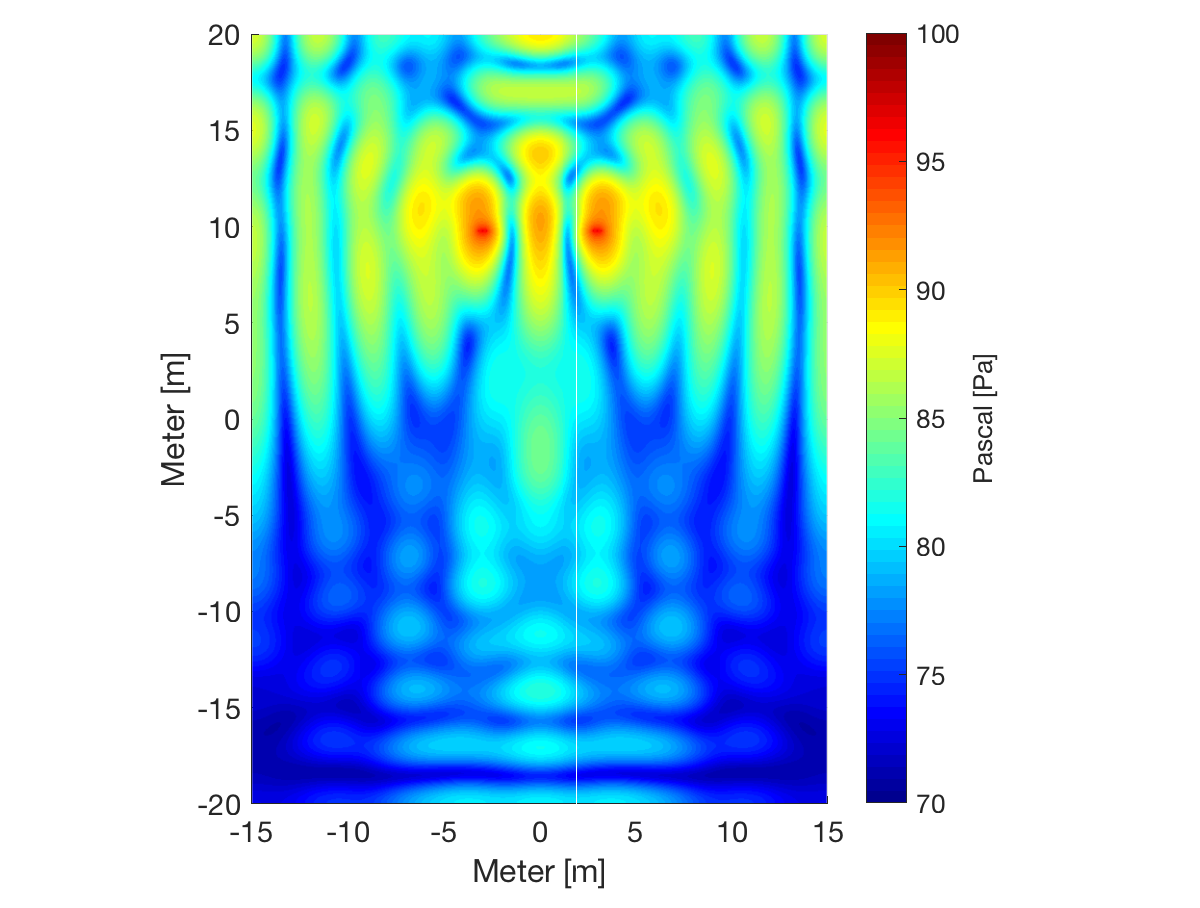
\includegraphics[width=0.95\textwidth]{60_hz_monitor_without_beam.eps}
\subcaption{Indoor simulation of  \SI{60}{\hertz} without beamforming}
\label{fig:Indoor_monitor_60_off}
\end{subfigure}\\
\hspace{0.1\textheight}
\begin{subfigure}[c]{0.5\textwidth}
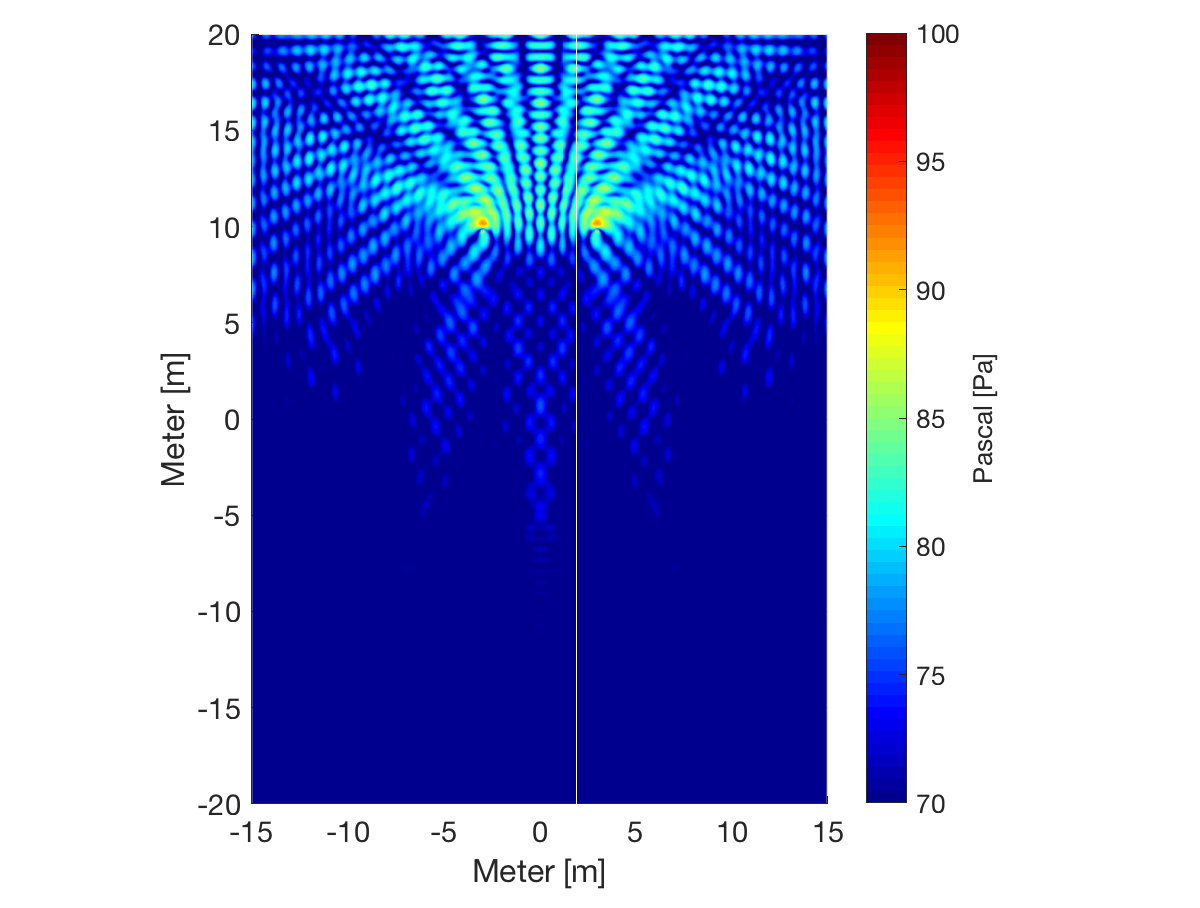
\includegraphics[width=0.95\textwidth]{300_hz_monitor_beam.eps}
\subcaption{Indoor simulation of  \SI{300}{\hertz} with beamforming}
\label{fig:Indoor_monitor_300_on}
\end{subfigure}
\begin{subfigure}[c]{0.5\textwidth}
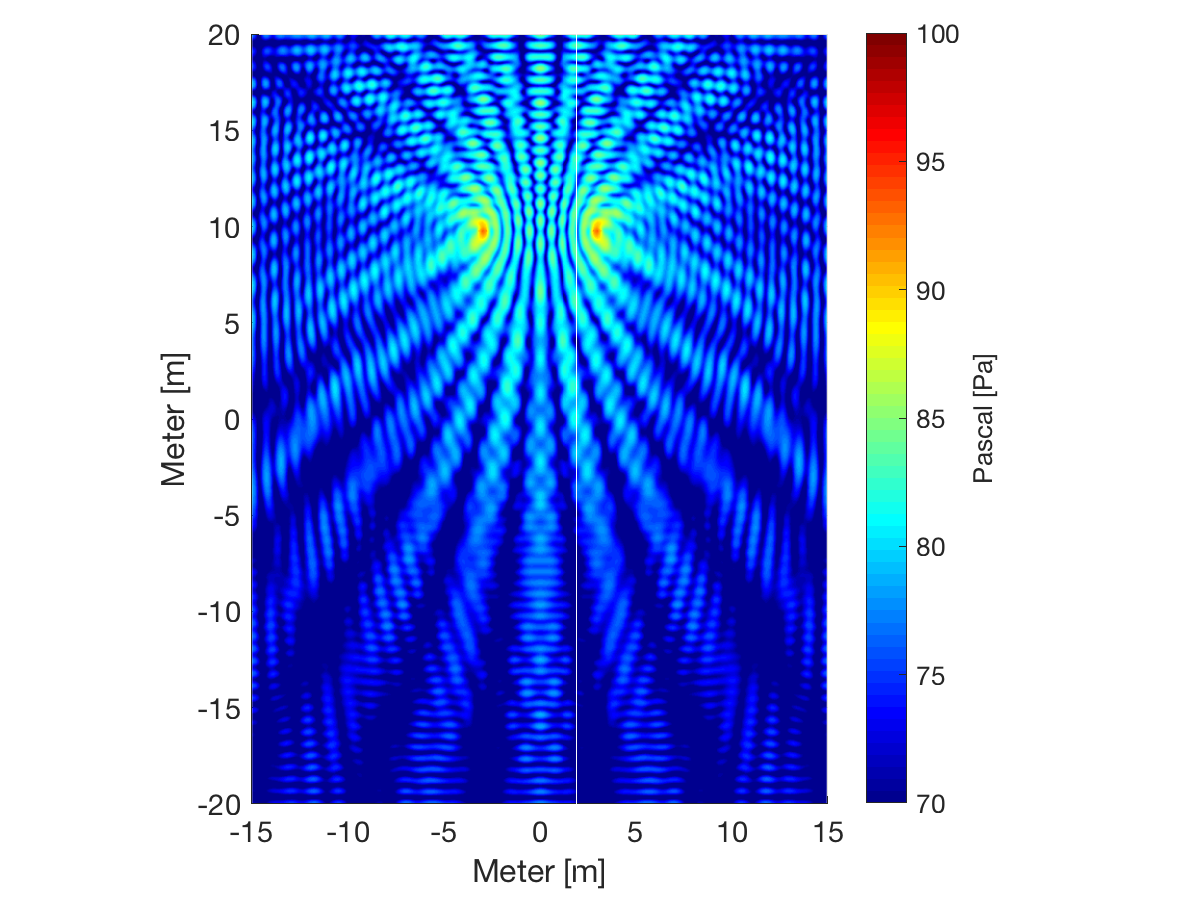
\includegraphics[width=0.95\textwidth]{300_hz_monitor_without_beam.eps}
\subcaption{Indoor simulation of  \SI{300}{\hertz} without beamforming}
\label{fig:Indoor_monitor_300_off}
\end{subfigure}
\caption{The figure shows a 2 dimension \gls{fdtd} simulation in a monitor application where the absorbing coefficient is set to 0.5}
		\label{fig:Indoor_monitor_60_300}
\end{figure}

In \autoref{fig:Indoor_monitor_60_300} it can be seen that the two monitoring arrays mostly reduce the sound pressure that is emitted towards the audience and do not change much on stage compared to the non-beamforming reference case. One way, the monitoring system might enhanced, could be that those two arrays are replaced by only one beamforming monitor, that is fed different signals with different beamforming processing. The main lobe of one of the signals signal could be pointed to the left of the monitor, and another one would be playing to the right. This concept has not been tested in this project, but it might be one possibility future investigations on the beamforming system.

